The analysis is performed under a blinded strategy to avoid bias in the interpretation of the results. This means that the data in the most sensitive signal regions is not inspected until the statistical model has been fully validated. Before unblinding, a series of dedicated fit studies is carried out using the blinded model to ensure that the any pulls in the model are understood and not a result of mis-modelling, and that the systematic uncertainties are properly implemented. After these studies we proceeded with the unblinding to reveal our signal contributions.\\
\\
This section will discuss the construction of statistical model and the fit studies conducted. A large number of fit studies were carried out between myself and the analysis team to validate the statistical model. I will briefly summarise a selection of these studies to illustrate the methodology and complexity of these studies. Finally, I present the validated, unblinded model that forms the basis of the measurement.
\subsection{Constructing the Model}
As mentioned in Chapter \ref{chap:AnalTech} the likelihood function is created within the RooStat framework \cite{roostats1,roostats2}, which is applied using TRExFitter, which is based on HistFactory \cite{histlab}. The minimisation is performed using the Minuit library implemented in ROOT \cite{minut,root}. The likelihood function used in this analysis is defined as the product of Poisson probabilities for each bin of the signal and background templates, given the observed data, together with Gaussian constraint terms that encode systematic uncertainties. Explicitly, the likelihood takes the form:
\begin{equation}
\mathcal{L}(\mu, \vec{k}, \vec{\theta}) = 
\prod_{r \in \{\text{SR, CR}\}}
\left[
\prod_{i \in \text{bins}} 
P \big( n_{r,i} \,|\, \nu_{r,i}(\mu, \vec{k}, \vec{\theta}) \big)
\right]
\times
\prod_{j \in \text{syst.}} 
G(\theta^0_j \,|\, \theta_j),
\label{eq:likelihood}
\end{equation}
where $n_{r,i}$ denotes the observed number of events in bin $i$ of region $r$, and $\nu_{r,i}$ the corresponding expected yield, which depends on the signal strength $\mu$, the background normalisation factors $\vec{k}$, 
and the nuisance parameters $\vec{\theta}$. All nuisance parameters $\theta_j$ are defined such that their best-fit values correspond to $\hat{\theta}_j \equiv \theta^0_j = 0$, with associated uncertainties normalised to unity ($\sigma_{\hat{\theta}} \equiv \Delta \theta = 1$). This convention effectively calibrates the likelihood. Finally, statistical uncertainties from the limited size of Monte Carlo simulated samples are included as additional Poisson terms.


\subsection{Fit Studies}
Here we detail two example fit studies conducted during the validation of the statistical model of the analysis which required additional investigation. These studies were performed on various versions of the fit. As such, steps were taken to relax tensions and pulls in the initial fits prior to the final fit. As, shown in Section \ref{final_model}, some pulls were relaxed. If pulls remain in the final fit these pull were well enough understood. Many other minor fit studies were conducted during this time most of which were simple decorrelations of NP to identify problem regions. The systematic variation plots were then inspected and either a change to the smoothing algorithm or implementing a newer version of CDI, which resulted in a relaxation of the pull. These minor studies are omitted for the sake of brevity.
\subsubsection{$t\bar{t}\geq2b$ PS PH7 Pull In The Single Lepton Channel}
A significant pull was observed in the single-lepton channel for the $t\bar{t}\geq 2b$ parton-shower PH7 (Powheg + Herwig 7) systematic. The presence of this pull indicated that the fit was using the nuisance parameter aggressively, suggesting non-trivial mismodelling effects. To identify the source, a systematic de-correlation across analysis regions was performed. This showed that the $t\bar{t}+c$ control region was the principal driver of the tension. The plots showing the pulls are shown below in Figure \ref{fig:tt2b_ps_PH7_pulls}.
\begin{figure}[!htb]
  \centering
  \begin{subfigure}{0.45\textwidth}
    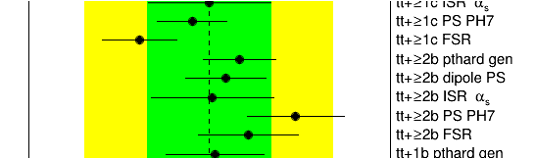
\includegraphics[width=\linewidth]{Section_tthbb_analysis/FIt_studies_figures/ttbb_ph7_pull.png}
    \caption{}
    \label{fig:first}
  \end{subfigure}
  \hfill
  \begin{subfigure}{0.45\textwidth}
    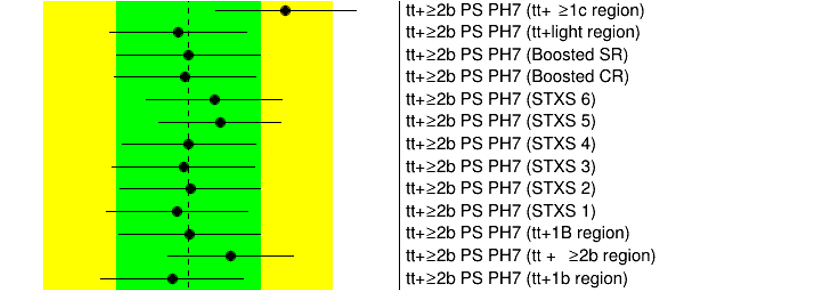
\includegraphics[width=\linewidth]{Section_tthbb_analysis/FIt_studies_figures/ttbb_ph7_pull_decorr.png}
    \caption{}
    \label{fig:second}
  \end{subfigure}
  \caption{Pull plots showing the $t\bar{t}+2b$ PS PH7 and $t\bar{t}+c$ FSR pull (a) the region decorrelation of the $t\bar{t}+2b$ PS PH7 pull (b).}
  \label{fig:tt2b_ps_PH7_pulls}
\end{figure}\\
\\
Inspection of the NP in this region revealed that the systematic had a pronounced shape effect rather than acting as a pure normalization shift. Comparison of pre- and post-fit distributions confirmed that data–MC discrepancies persisted even after the fit, reinforcing the hypothesis that the pull was rooted in shape mismodelling. To probe this further, the behaviour of $t\bar{t}+2b$ events within the $t\bar{t}+c$ control region was examined shown in Figure \ref{fig:ttbb_ps_ph7_red_blue}.
\begin{figure}[!htb]
  \centering
    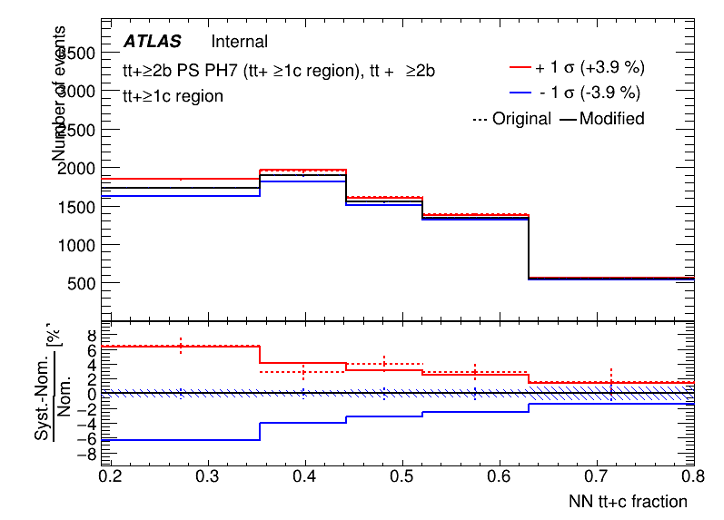
\includegraphics[width=0.6\linewidth]{Section_tthbb_analysis/FIt_studies_figures/ttbb_ph7_ttc_red_blue.png}
  \caption{The systematic variation plot $t\bar{t}\geq 2b$ parton-shower PH7 systematic in the $t\bar{t}+2b$ sample in the $t\bar{t}+c$.}
  \label{fig:ttbb_ps_ph7_red_blue}
\end{figure}\\
\\
The $t\bar{t}\geq2b$ contribution exhibited a clear shape modification: the yield was enhanced at low NN($t\bar{t}+c$) scores in a way that closely followed the behaviour of the PH7 systematic. At higher NN scores, additional systematics appeared to be involved, indicating that the tension was not attributable to a single nuisance. Several candidate systematics, acting both on $t\bar{t}+c$ and $t\bar{t}+2b$ samples, were identified as capable of amplifying the apparent $t\bar{t}+2b$ contribution, particularly in the high-NN bins.
\begin{figure}[!htb]
  \centering
    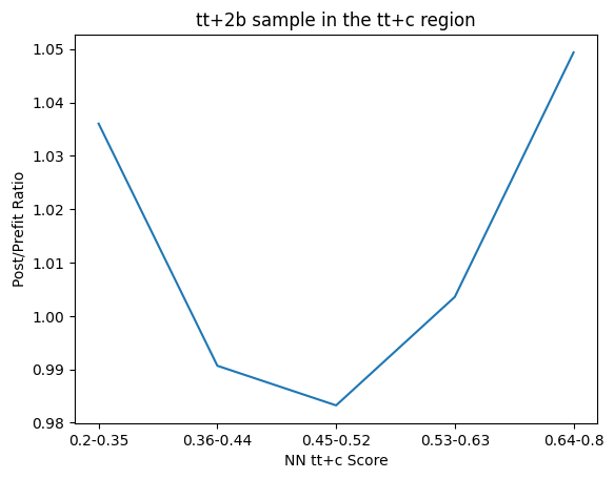
\includegraphics[width=0.6\linewidth]{Section_tthbb_analysis/FIt_studies_figures/ttbb_sample_ttc_region_preprost.png}
  \caption{A distribution of the $t\bar{t}+2b$ sample in the $t\bar{t}+c$ region as a function of NN  $t\bar{t}+c$ score.}
  \label{fig:light_EV0_red_blue}
\end{figure}
Further evidence came from the $t\bar{t}+c$ FSR systematic, which also showed a strong pull and introduced noticeable shape distortions shown in Figure \ref{fig:tt2b_ps_PH7_pulls}. This suggests that multiple, entangled nuisance parameters propagate through the fit, combining to produce the observed PH7 pull. In short, the $t\bar{t}+2b$ PH7 systematic does not reflect a single isolated modelling issue but rather the interplay of overlapping systematics in the $t\bar{t}+c$ control region. We also see that the raw systematic variation plots for $t\bar{t}+2b$ FSR and dipole systematics, shown in Figure \ref{fig:tt2b_FSR_dipole}, for the $t\bar{t}+2b$ sample in the $t\bar{t}+c$ region, show the possible increase in $t\bar{t}+2b$ events in the $t\bar{t}+c$ region at high $t\bar{t}+c$ NN score bins. This plays into the non trivial nature of the $t\bar{t}+2b$ PS PH7 systematic.
\begin{figure}[!htb]
  \centering
  \begin{subfigure}{0.45\textwidth}
    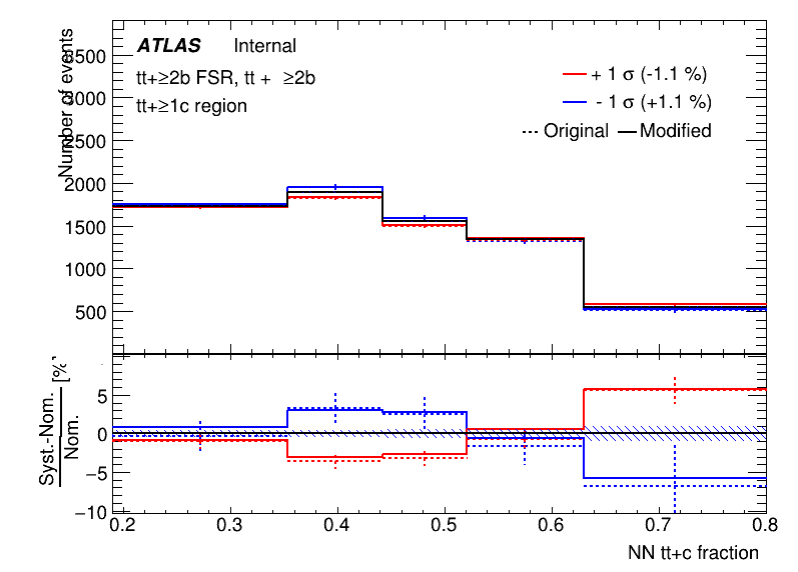
\includegraphics[width=\linewidth]{Section_tthbb_analysis/FIt_studies_figures/ttbb_FSR_ttc.png}
    \caption{}
    \label{fig:first}
  \end{subfigure}
  \hfill
  \begin{subfigure}{0.45\textwidth}
    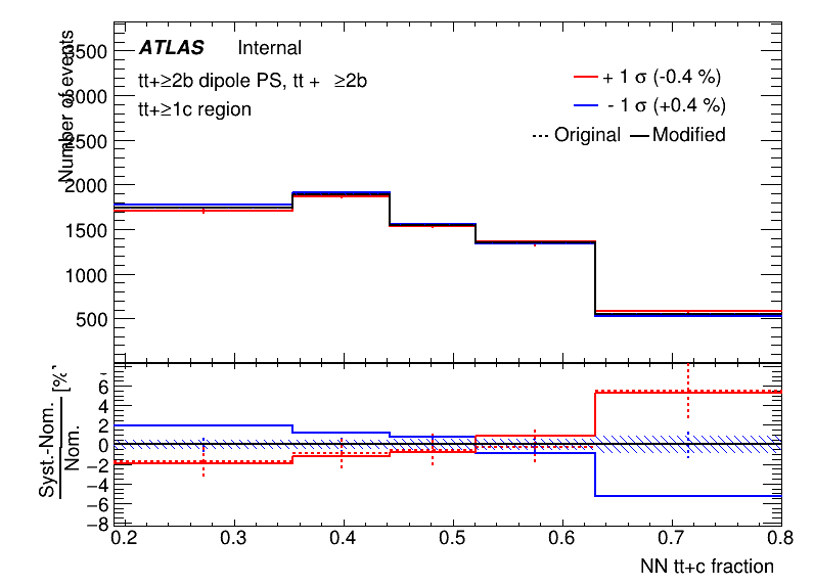
\includegraphics[width=\linewidth]{Section_tthbb_analysis/FIt_studies_figures/ttbb_dipole_ttc.png}
    \caption{}
    \label{fig:second}
  \end{subfigure}
  \caption{The systematic variation plots for $t\bar{t}+2b$ FSR (a) and dipole (b) systematics for the $t\bar{t}+2b$ sample in the $t\bar{t}+c$ region.}
  \label{fig:tt2b_FSR_dipole}
\end{figure}
\subsubsection{Flavour Tagging Light EV0 Pull}
In the combined fit, a moderate but non-negligible pull was observed in the light-jet EV0 systematic, shown in Figure \ref{fig:light_EV0_pull}. Importantly, this behaviour was absent in the individual single-lepton and di-lepton fits, but appeared only in the combination. The presence of such a pull indicates that the fit is using this nuisance parameter to absorb tension between channels, rather than correcting a feature of the data.
\begin{figure}[!htb]
  \centering
    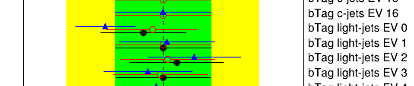
\includegraphics[width=0.7\linewidth]{Section_tthbb_analysis/FIt_studies_figures/light_EV0_pull.png}

  \caption{Pull plots showing the flavour tagging light jet EV0 pull in the combination fit.}
  \label{fig:light_EV0_pull}
\end{figure}\\
\\
The first step was to inspect the pre-fit and post-fit behaviour of the $t\bar{t}+\text{light}$ control region. The di-lepton channel showed higher yield and larger variation than the single lepton channel, suggesting that the fit was exploiting the EV0 nuisance to balance the two. At first this was thought to be an implementation error. However, considering the event definition of each channel revealed an important difference: in the single lepton selection, the hadronic $W$ decay can proceed via $W \to cs$, introducing a charm quark that is more likely to be mis-tagged as a $b$-jet. This mechanism effectively reduces the relative rate of light-jet mis-tags in the single lepton sample. By contrast, in the di-lepton channel both $W$ bosons decay leptonically, so this source of charm contamination is absent, making the di-lepton channel more sensitive to genuine light-jet mis-tagging. The result is an intrinsic difference between the two channels in their response to the EV0 systematic. The systematic variation plots for the light EV0 systematic in the single and di-lepton channel for in the $tt+$light region is shown in Figure \ref{fig:light_EV0_red_blue}.
\begin{figure}[!htb]
  \centering
  \begin{subfigure}{0.45\textwidth}
    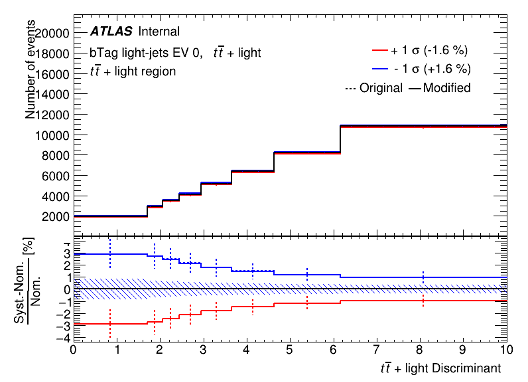
\includegraphics[width=\linewidth]{Section_tthbb_analysis/FIt_studies_figures/light_EV0_tt_light_1l.png}
    \caption{}
    \label{fig:first}
  \end{subfigure}
  \hfill
  \begin{subfigure}{0.45\textwidth}
    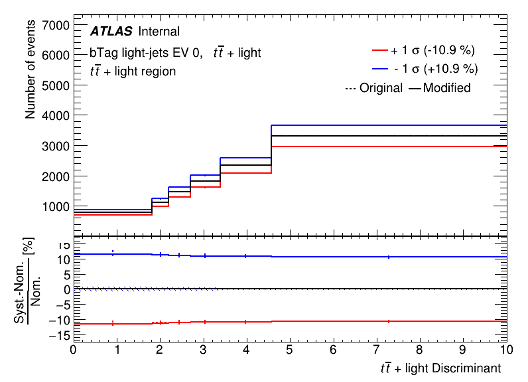
\includegraphics[width=\linewidth]{Section_tthbb_analysis/FIt_studies_figures/light_EV0_tt_light_2l.png}
    \caption{}
    \label{fig:second}
  \end{subfigure}
  \caption{The systematic variation plots for the light EV0 systematic in the single (a) and di-lepton (b) channel for the $t\bar{t}+$light region.}
  \label{fig:light_EV0_red_blue}
\end{figure}\\
\\
Comparing the behaviour of the $c$-jet EV0 nuisance across channels. Indeed, the single lepton channel showed stronger sensitivity to $c$-jet mis-tags, consistent with the $W \to cs$ contribution, whereas the di-lepton channel retained a stronger dependence on light-jet mistagging. This confirmed that the channel-specific physics was driving the tension.
\begin{figure}[!htb]
  \centering
  \begin{subfigure}{0.45\textwidth}
    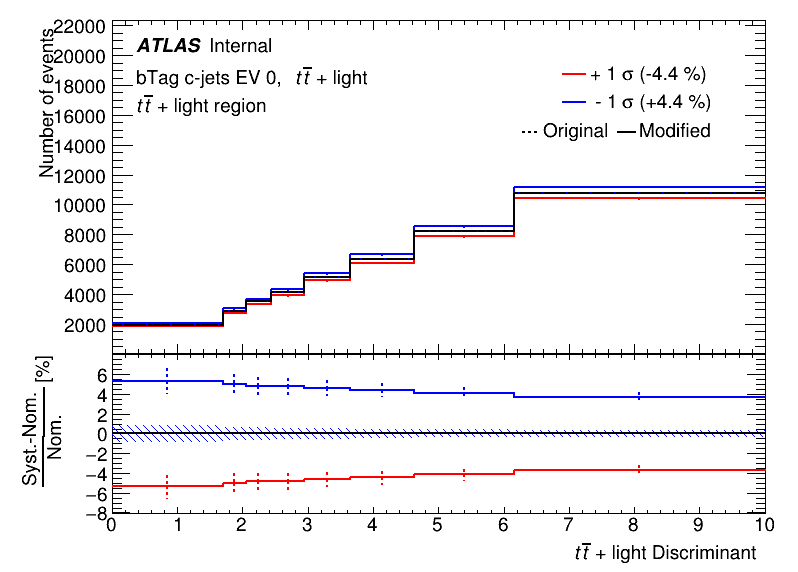
\includegraphics[width=\linewidth]{Section_tthbb_analysis/FIt_studies_figures/c_EV0_tt_light_1l.png}
    \caption{}
    \label{fig:first}
  \end{subfigure}
  \hfill
  \begin{subfigure}{0.45\textwidth}
    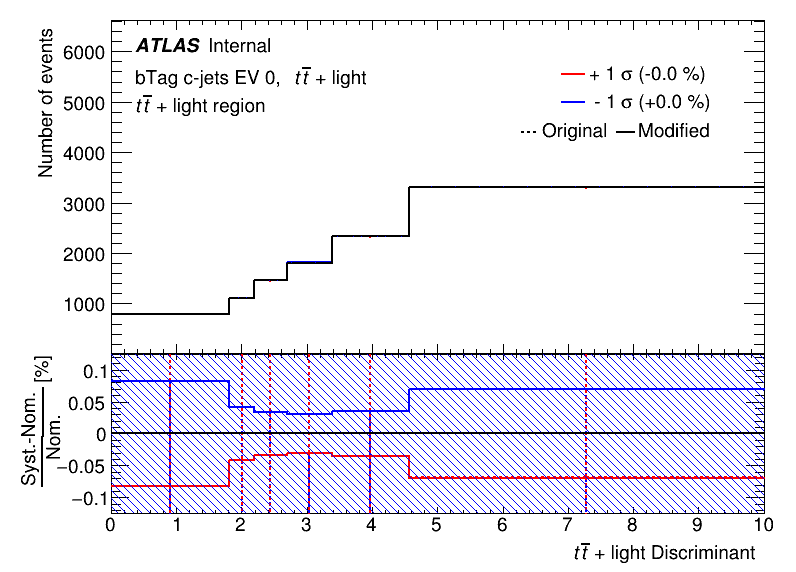
\includegraphics[width=\linewidth]{Section_tthbb_analysis/FIt_studies_figures/c_EV0_tt_light_2l.png}
    \caption{}
    \label{fig:second}
  \end{subfigure}
  % \hfill
  % \begin{subfigure}{0.32\textwidth}
  %   \includegraphics[width=\linewidth]{fig3.pdf}
  %   \caption{Third figure}
  %   \label{fig:third}
  % \end{subfigure}
  \caption{The systematic variation plots for the $c$-jets EV0 systematic in the single (a) and di-lepton (b) channel in the $t\bar{t}+$light region.}
  \label{fig:three-side}
\end{figure}\\
\\
Finally, we explored whether the pull could be relaxed by de-correlating the $k$-factors associated with the $t\bar{t}+\text{light}$ background across the two channels. Allowing $k_{t\bar{t}+\text{light}}^{1\ell}$ and $k_{t\bar{t}+\text{light}}^{2\ell}$ to float independently reduced the combined light-jet EV0 pull to below one standard deviation. This shows that the nuisance parameter was previously acting as a proxy to reconcile mismodelling differences between the channels, rather than indicating a fundamental problem with the flavour-tagging implementation. This study was shown to the flavour tagging group who agreed that this was a feature of the fit and not a bug in the derivation of the NPs.
\begin{figure}[!htb]
    \centering
    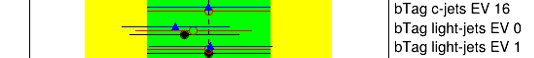
\includegraphics[width=0.7\linewidth]{Section_tthbb_analysis/FIt_studies_figures/light_EV0_pull_RELAXED.png}
    \caption{The relaxed pull of the light EV0 systematic.}
    \label{fig:placeholder}
\end{figure}\\
\\
This decorrelated $k$-factor approach, based on my recommendation, was adopted as in the final fit as shown in Figure \ref{fig:background norm}. 

\subsection{Finalised Statistical Model}
\label{final_model}
The finalised statistical model represented by the $S+B$ fit showing the background normalisation factors in Figure \ref{fig:background norm}. The $t\bar{t}$ specific background modelling systematic pulls in Figure \ref{ttbar_pulls_final}. The flavour tagging systematic pulls, Figure \ref{fig:flavou_pulls}. The number of finalised extrapolation uncertainties presented in Chapter \ref{chap:PCBTextrap} and seen in the final fit are different due to some being pruned out. Finally, we have the other modelling systematic parameters shown in Figure \ref{fig:fitstudies_modelling}.
\begin{figure}[!htb]
    \centering
    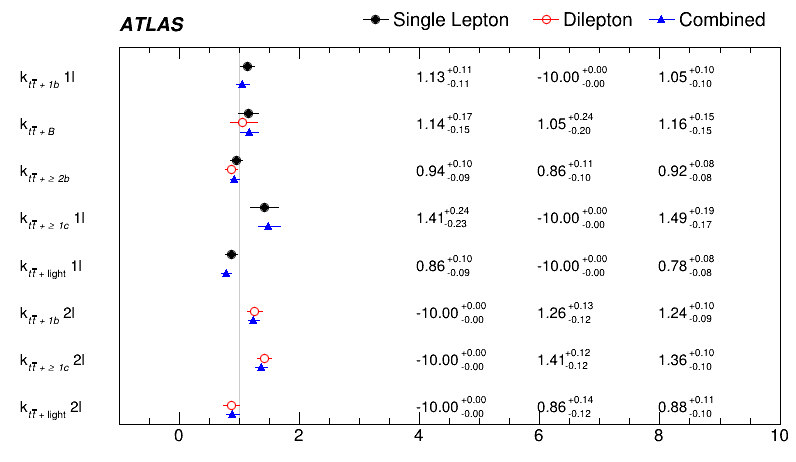
\includegraphics[width=1\linewidth]{Section_tthbb_analysis/figures/Final_fit/NormFactors_comp.png}
    \caption{Best-fit results for all free-floating normalization factors in a fit to observed data. The background normalization factor comparison includes fits to only the single lepton and di-lepton channels, respectively, as well as the combined fit to all channels. Entries of -10 indicate that the normalization factor is not defined.}
    \label{fig:background norm}
\end{figure}
 \begin{figure}[!htb]
        \centering
            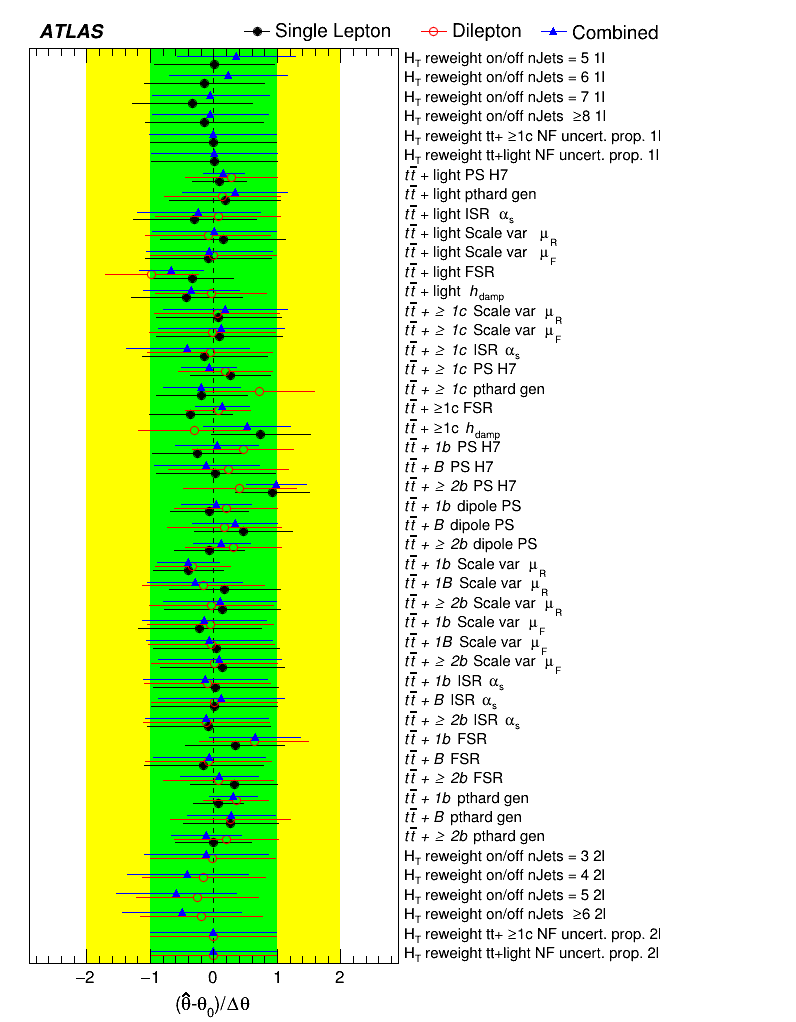
\includegraphics[width=1\linewidth]{Section_tthbb_analysis/figures/Final_fit/NuisPar_comp_Modelling_ttbar.png}
            \caption{The $t\bar{t}$ specific background modelling parameters pull plots for the final fit.}
            \label{ttbar_pulls_final}
    \end{figure}
\begin{figure}[!htb]
    \centering
    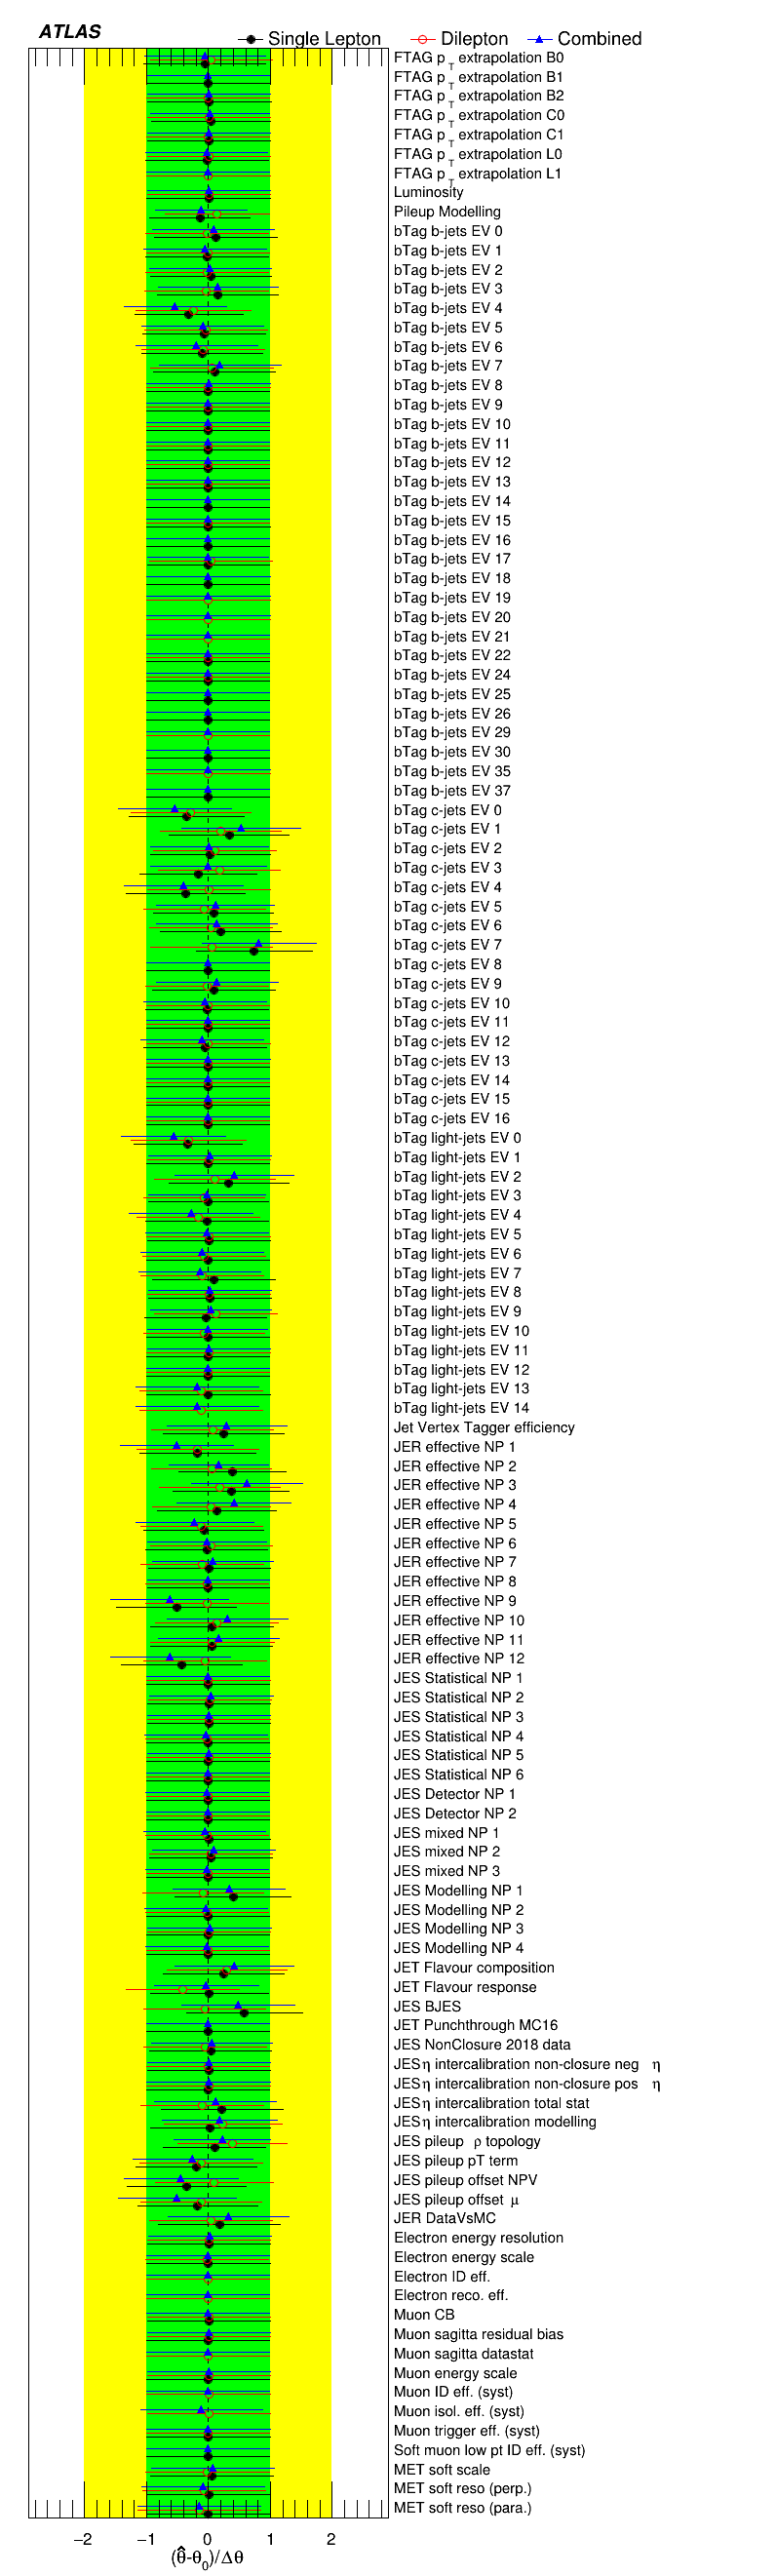
\includegraphics[width=0.4\linewidth]{Section_tthbb_analysis/figures/Final_fit/NuisPar_comp_Instrumental.png}
    \caption{The flavour tagging systematic pulls.}
    \label{fig:flavou_pulls}
\end{figure}
\begin{figure}[htbp]
    \centering
    \begin{minipage}{0.9\textwidth}
        \centering
        \begin{subfigure}{\linewidth}
            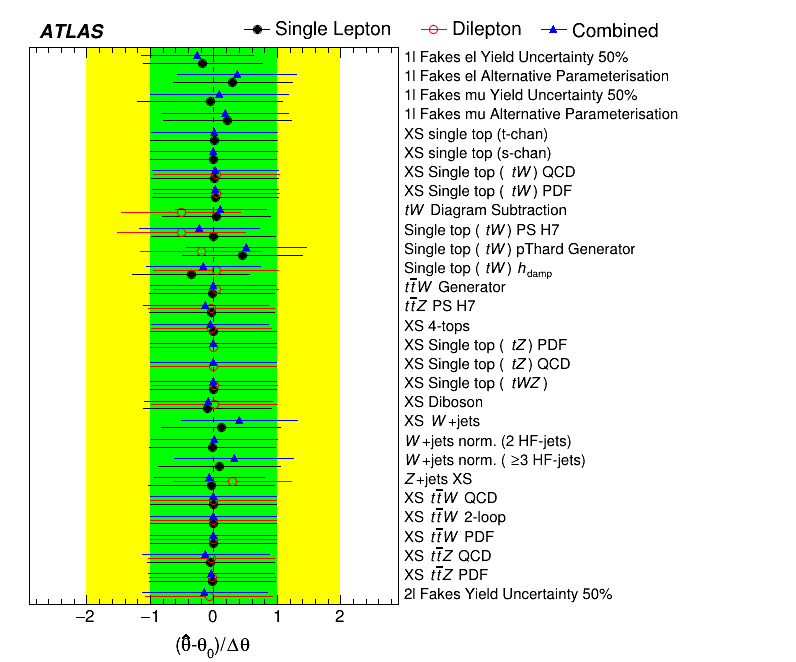
\includegraphics[width=\linewidth]{Section_tthbb_analysis/figures/Final_fit/NuisPar_comp_Modelling_other.png}
            \caption{}
        \end{subfigure}
        \vspace{0.3cm}
        
        \begin{subfigure}{\linewidth}
            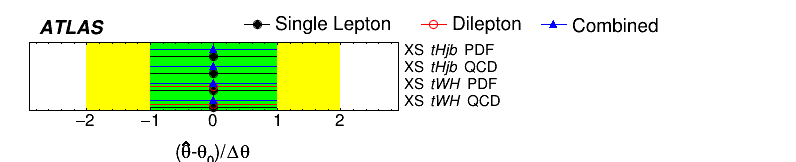
\includegraphics[width=\linewidth]{Section_tthbb_analysis/figures/Final_fit/NuisPar_comp_Modelling_tH.png}
            \caption{}
        \end{subfigure}
        \vspace{0.3cm}
        
        \begin{subfigure}{\linewidth}
            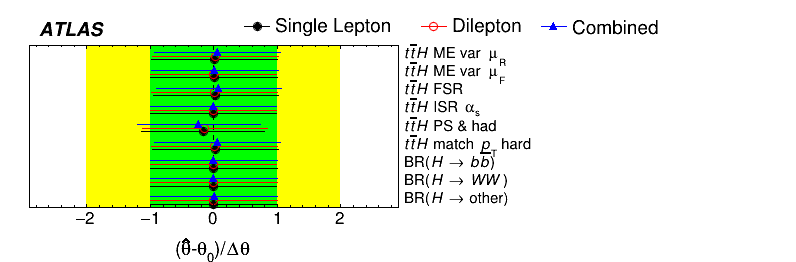
\includegraphics[width=\linewidth]{Section_tthbb_analysis/figures/Final_fit/NuisPar_comp_Modelling_ttH.png}
            \caption{}
        \end{subfigure}
    \end{minipage}    
    \caption{Nuisance parameter pulls across modelling categories: 
    (a) Other processes, (b) $tH$, (c) $t\bar{t}H$, and (d) $t\bar{t}$.}
    \label{fig:fitstudies_modelling}
\end{figure}



% \subsection{$t\bar{t}+\geq 2b$ PS Systematic in the Single-Lepton Channel}

% A large post-fit pull was observed in the $t\bar{t}+\geq 2b$ PS systematic when fitting the single-lepton channel.  
% \begin{figure}[h!]
%     \centering
%     \includegraphics[width=0.7\textwidth]{figures/FitStudies/ttbbPS_pull.pdf}
%     \caption{Post-fit pulls for the $t\bar{t}+\geq 2b$ PS systematic in the single-lepton channel.  
%     The $t\bar{t}+c$ control region drives the observed behaviour.}
%     \label{fig:fitstudies_ttbbPS}
% \end{figure}
% De-correlation of the systematic across regions revealed that the $t\bar{t}+c$ control region was the primary source of this behaviour.  

% \begin{figure}[h!]
%     \centering
%     \includegraphics[width=0.7\textwidth]{figures/FitStudies/ttbbPS_pull.pdf}
%     \caption{Post-fit pulls for the $t\bar{t}+\geq 2b$ PS systematic in the single-lepton channel.  
%     The $t\bar{t}+c$ control region drives the observed behaviour.}
%     \label{fig:fitstudies_ttbbPS}
% \end{figure}


% Closer inspection showed a shape discrepancy in the $t\bar{t}+2b$ contribution within this region. The systematic appeared to drive an enhanced $t\bar{t}+2b$ yield in the lower bins of the $t\bar{t}+c$ neural network discriminant, and also influenced the highest-scoring bins.  
% Additional contributions were traced to the $t\bar{t}+c$ FSR systematic, which exhibited a sizeable pull and further distorted the shape.  
% Overall, the $t\bar{t}+c$ region displayed multiple shape effects that propagated through the fit, leading to compensating pulls in related nuisance parameters.  

% \subsection{Combined $t\bar{t}+1b$ Dipole PS Systematic}

% A second large pull was found in the dipole PS systematic affecting the $t\bar{t}+1b$ background, but only in the combined fit.  
% De-correlation studies indicated that this was driven primarily by the $t\bar{t}+1b$ regions.  
% A key feature was the difference in fitted normalisation factors across the channels: in the single-lepton channel, the fitted $k$-factor was $0.88^{+0.11}_{-0.10}$, while in the dilepton channel it was $1.31^{+0.26}_{-0.21}$.  
% The combined fit resulted in a $k$-factor of $1.08^{+0.11}_{-0.10}$, with the nuisance parameter absorbing part of the tension between the two channels.  
% This behaviour suggests that the systematic is compensating for the channel-dependent normalisation differences, rather than reflecting a genuine modelling effect.  

% \subsection{Discussion}

% Both cases underline the sensitivity of the fit to mismodelling in specific control regions.  
% For the $t\bar{t}+c$ region, shape mismodelling in $t\bar{t}+2b$ and FSR variations appear to drive correlated pulls, while in the $t\bar{t}+1b$ case the dipole PS systematic absorbs tension between channels with inconsistent normalisation corrections.  
% Further studies, such as removing the normalisation component of the problematic systematics in the $t\bar{t}+c$ region and refitting, are suggested to better isolate the impact of these effects.  
 
